\documentclass[11pt,a4paper]{article}
\usepackage{fontspec}
\setmainfont{TeX Gyre Pagella}
\newfontfamily\headfont{Inter}[UprightFont=*-ExtraBold,BoldFont=*-ExtraBold,Extension=.otf,Path=/usr/share/fonts/opentype/inter/]
\usepackage[a4paper,margin=2.3cm]{geometry}
\usepackage{graphicx,booktabs,float,caption,array,xcolor,longtable}
\usepackage[hidelinks]{hyperref}
\usepackage{titlesec}
\usepackage[round]{natbib}
\usepackage{setspace}
\setstretch{1.05}
\renewcommand{\topfraction}{0.9}
\renewcommand{\bottomfraction}{0.8}
\renewcommand{\textfraction}{0.1}
\renewcommand{\floatpagefraction}{0.75}
\setlength{\parindent}{0pt}
\setlength{\parskip}{0.55em}
\titleformat{\section}{\headfont\Large}{\thesection}{0.8em}{}
\titleformat{\subsection}{\headfont\large}{\thesubsection}{0.8em}{}
\captionsetup{font=small,labelfont=bf}
\urlstyle{same}
\hypersetup{pdftitle={Holy Islands: Monks, Hermits and the Edge of the World},pdfauthor={Tristan Hotham}}

\begin{document}
\begin{center}
{\Large\bfseries Holy Islands\par}
\vspace{0.4em}
{\large Monks, hermits and the edge of the world: island monasteries in Wikidata, mapped through time\par}
\vspace{1.2em}
{\large Tristan Hotham\par}
\vspace{0.3em}
{\small Independent researcher\\
ORCID: 0000-0003-4931-9349\\
DOI: \href{https://doi.org/10.5281/zenodo.23844515}{https://doi.org/10.5281/zenodo.23844515}\par}
\vspace{0.8em}
2026
\end{center}

\begin{quote}
\small
\begin{center}\textbf{Abstract}\end{center}
Early medieval monks of the Atlantic edge of Europe are famous for seeking islands, from Iona and Lindisfarne to Bardsey and Skellig Michael. I test how distinctive that was using the 20,228 monasteries, abbeys, priories, convents, friaries and hermitages in Europe that Wikidata records with coordinates, placing each on the GSHHG full-resolution shoreline and treating land under 1,000 km$^2$ as island and Great Britain, Ireland and larger islands as mainland. 459 houses (2.3\%) stand on islands: 414 at sea and 45 in lakes and rivers. Among the 7,071 houses with a foundation date, the island share falls from 4.3\% before 800 to 1.1\% for 1100 to 1299 and 1.2\% thereafter. On the Atlantic Celtic edge (Ireland, Scotland, Wales, Brittany, Galicia), 3 of 28 houses dated before 1100 are on islands (10.7\%, 95\% interval 3.7 to 27.2\%), against 5 of 3,230 (0.2\%) founded in France and Central Europe from 1100. The island houses furthest from the mainland are the early modern convents of the Azores, up to 1,656 km out. Of 2,944 dated closures, 614 fall in England and Wales in 1536 to 1541; the Viking raids leave no trace in the record. Coverage is very uneven: only 35\% of houses are dated and Germany holds 24\% of them.

\textbf{Keywords:} monasticism; islands; early medieval; Insular Christianity; Dissolution of the Monasteries; Wikidata; GSHHG; historical geography
\end{quote}

\section{Introduction}
Among the most familiar images of early medieval Christianity are its island monasteries: the beehive cells of Skellig Michael on a rock off Kerry, Columba's Iona, Aidan's Lindisfarne, the twenty thousand saints said to lie on Bardsey. Irish and British monks of the sixth to eighth centuries sought a `desert in the ocean', and some, according to Dicuil writing around 825, reached the Faroes and Iceland before the Norse \citep{dicuil}. The idea was older and wider: Honoratus founded his community on the Lérins islands off Cannes around 410, and lake islands such as Reichenau carried the same logic inland.

How distinctive was this? Histories of monasticism tend to proceed by famous cases, and the famous cases are islands. This study asks a simple quantitative question of an open, Europe-wide record: what share of known monastic houses stand on islands, and does the share change by date of foundation and by region? It also asks which island houses lie furthest from the mainland, and when houses were dissolved or abandoned.

The source is Wikidata \citep{wikidata}, whose monastery records come from many national heritage lists and from Wikipedia editors. It is broad but uneven, and much of this paper is about the limits that this places on the answers. An interactive map accompanies the paper (\url{https://maps.tristanhotham.com/holy-islands/}).

\section{Data}
\textbf{Monastic houses.} Every Wikidata item that is an instance of a subclass of monastery (Q44613), hermitage (Q513550), abbey (Q160742), priory (Q2750108) or clochán (Q1175763) and has coordinates, retrieved through QLever \citep{qlever} in 2026: 36,745 result rows for 29,874 items worldwide. For each item I kept its English label (70\% of houses in the study area have one), point, classes, country, number of sitelinks, and the earliest inception (P571) and dissolved or abandoned (P576) dates.

\textbf{Study area.} Europe in the broad sense: Natural Earth's European countries plus Cyprus and Turkey, west of 60\textdegree{}E, including Iceland, the Faroes and Macaronesia \citep{naturalearth}. I dropped 136 items whose only classes are not monastic houses (wayside shrines, lodgings such as the auberges of Valletta, town houses of abbeys, an abbot's palace) or are Buddhist monasteries, leaving 20,228 houses in 45 countries.

\textbf{Shorelines.} GSHHG, the Global Self-consistent, Hierarchical, High-resolution Geography database \citep{gshhg}, at full resolution, as packaged in the basemap-data-hires Python package. Its hierarchy separates land, lakes and islands in lakes, and it includes islets of well under one square kilometre (Skellig Michael's island is 0.5 km$^2$ in it).

\begin{table}[tbp]\centering\small\caption{Sources, what was kept and licences.}\label{tab:sources}\begin{tabular}{>{\raggedright\arraybackslash}p{3.0cm}>{\raggedright\arraybackslash}p{7.4cm}r>{\raggedright\arraybackslash}p{2.0cm}}\toprule Source & Kept & Records & Licence\\\midrule
Wikidata & Monastic houses with coordinates, worldwide & 29,874 & CC0\\
Wikidata & Houses in the study area (Europe) & 20,228 & CC0\\
Wikidata & of which with a foundation date (P571) & 7,071 & CC0\\
Wikidata & of which with a dissolution date (P576) & 2,944 & CC0\\
GSHHG & Full-resolution land, lake and lake-island polygons & 178 with houses & LGPL-3.0\\
Natural Earth & Countries, provinces, populated places & & Public domain\\
\bottomrule\end{tabular}\end{table}

\section{Methods}
\subsection{Islands}
Each point was tested against the GSHHG polygons. A point on an island in a lake (level 3) is a lake island. A point in a lake but not on a mapped lake island is moved to a lake island within 1.5 km if there is one, otherwise left on the surrounding land. A point in the sea within 1.5 km of land is put on that land; 2 points further out could not be placed.

An island is land under 1,000 km$^2$. Continental Eurasia and Africa, Great Britain, Ireland and every other island of 1,000 km$^2$ or more (Iceland, Sicily, Sardinia, Corsica, Crete, Cyprus, Zealand, Gotland, Mallorca, Lewis and Harris and others) are treated as mainland, since a house there was not choosing an island in any meaningful sense. Counting the 429 houses on those larger islands as island houses would raise the overall share from 2.3\% to 4.4\%. Islands under 25 km$^2$, the scale of Iona, Lindisfarne and Bardsey, are reported separately as small islands.

The shoreline data miss many small islands in lakes and rivers. I flagged every house whose English label names an island (46 houses: Island, Isle, Inis, Inish, Inch, Ynys, Eilean, Île, Insel and similar) and checked by hand those the shoreline placed on the mainland. 16 were moved onto lake or river islands (for example Inis Cealtra in Lough Derg, Inchmahome in the Lake of Menteith, Margaret Island in the Danube) and two onto sea islets missing from GSHHG (Church Island in Valentia Harbour; Kiy Island in the White Sea). Houses whose names contain a town name (L'Isle, L'Île-Bouchard) or that stood on islands since joined to the land (Inch Abbey, Inchaffray, St Peter's Island in Lake Biel) were left on the mainland: the classification is of present geography. Of the flagged houses, 30 (65\%) end up on islands; conversely only 7\% of island houses have an island word in their label, so names alone would find very few.

Distance from the mainland is measured from each sea-island house to the nearest coast of continental Europe, Africa, Great Britain or Ireland, in the LAEA Europe projection; for lake islands, to the lake shore.

\subsection{Dates, periods and regions}
Inception is the date a house was founded, which for a refounded house is often its last refoundation. Wikidata stores dates of century precision as full dates, and the extract does not carry the precision: the excess of 1 January dates in years ending 00 and 01 shows this. I read years ending in 01 on 1 January as the middle of the century they begin (1101 as 1150) and years ending in 00 on 1 January as the middle of the century they end (1100 as 1050); 28\% of dates are of this kind. The alternative reading of 00 years is reported as a sensitivity check. 8 inception dates later than 2026 were treated as missing.

Houses were grouped into four periods by date of foundation (before 800; 800 to 1099; 1100 to 1299; 1300 and later) and into thirteen regions from their country and the Natural Earth province: the five regions of the Atlantic Celtic edge (Ireland, north and south; Scotland; Wales; historic Brittany, the five departments; Galicia) and England with Man and the Channel Islands, the rest of France, the rest of Iberia, Iceland and the Faroes, Scandinavia and the Baltic, Central Europe and the Low Countries, the Mediterranean (Italy, Malta, Greece, Cyprus, Turkey, the Adriatic states, Provence, Corsica, Catalonia, Valencia, Murcia and the Balearics) and Eastern Europe and the Balkans. Shares carry Wilson 95\% intervals.

\section{Results}
\subsection{How many houses stand on islands}
459 of 20,228 houses (2.3\%) stand on islands under 1,000 km$^2$ (Figure~\ref{fig:map}): 107 on small sea islands, 307 on larger sea islands and 45 on islands in lakes and rivers. They sit on 178 distinct mapped islands. The islands with most houses are in the Aegean: 37 on Imbros (Gökçeada) 16 on Paros and 14 on Chios, with Corfu, Naxos and Andros close behind; Valaam in Lake Ladoga has 10, counting its sketes, and Reichenau 8.

\begin{figure}[tbp]\centering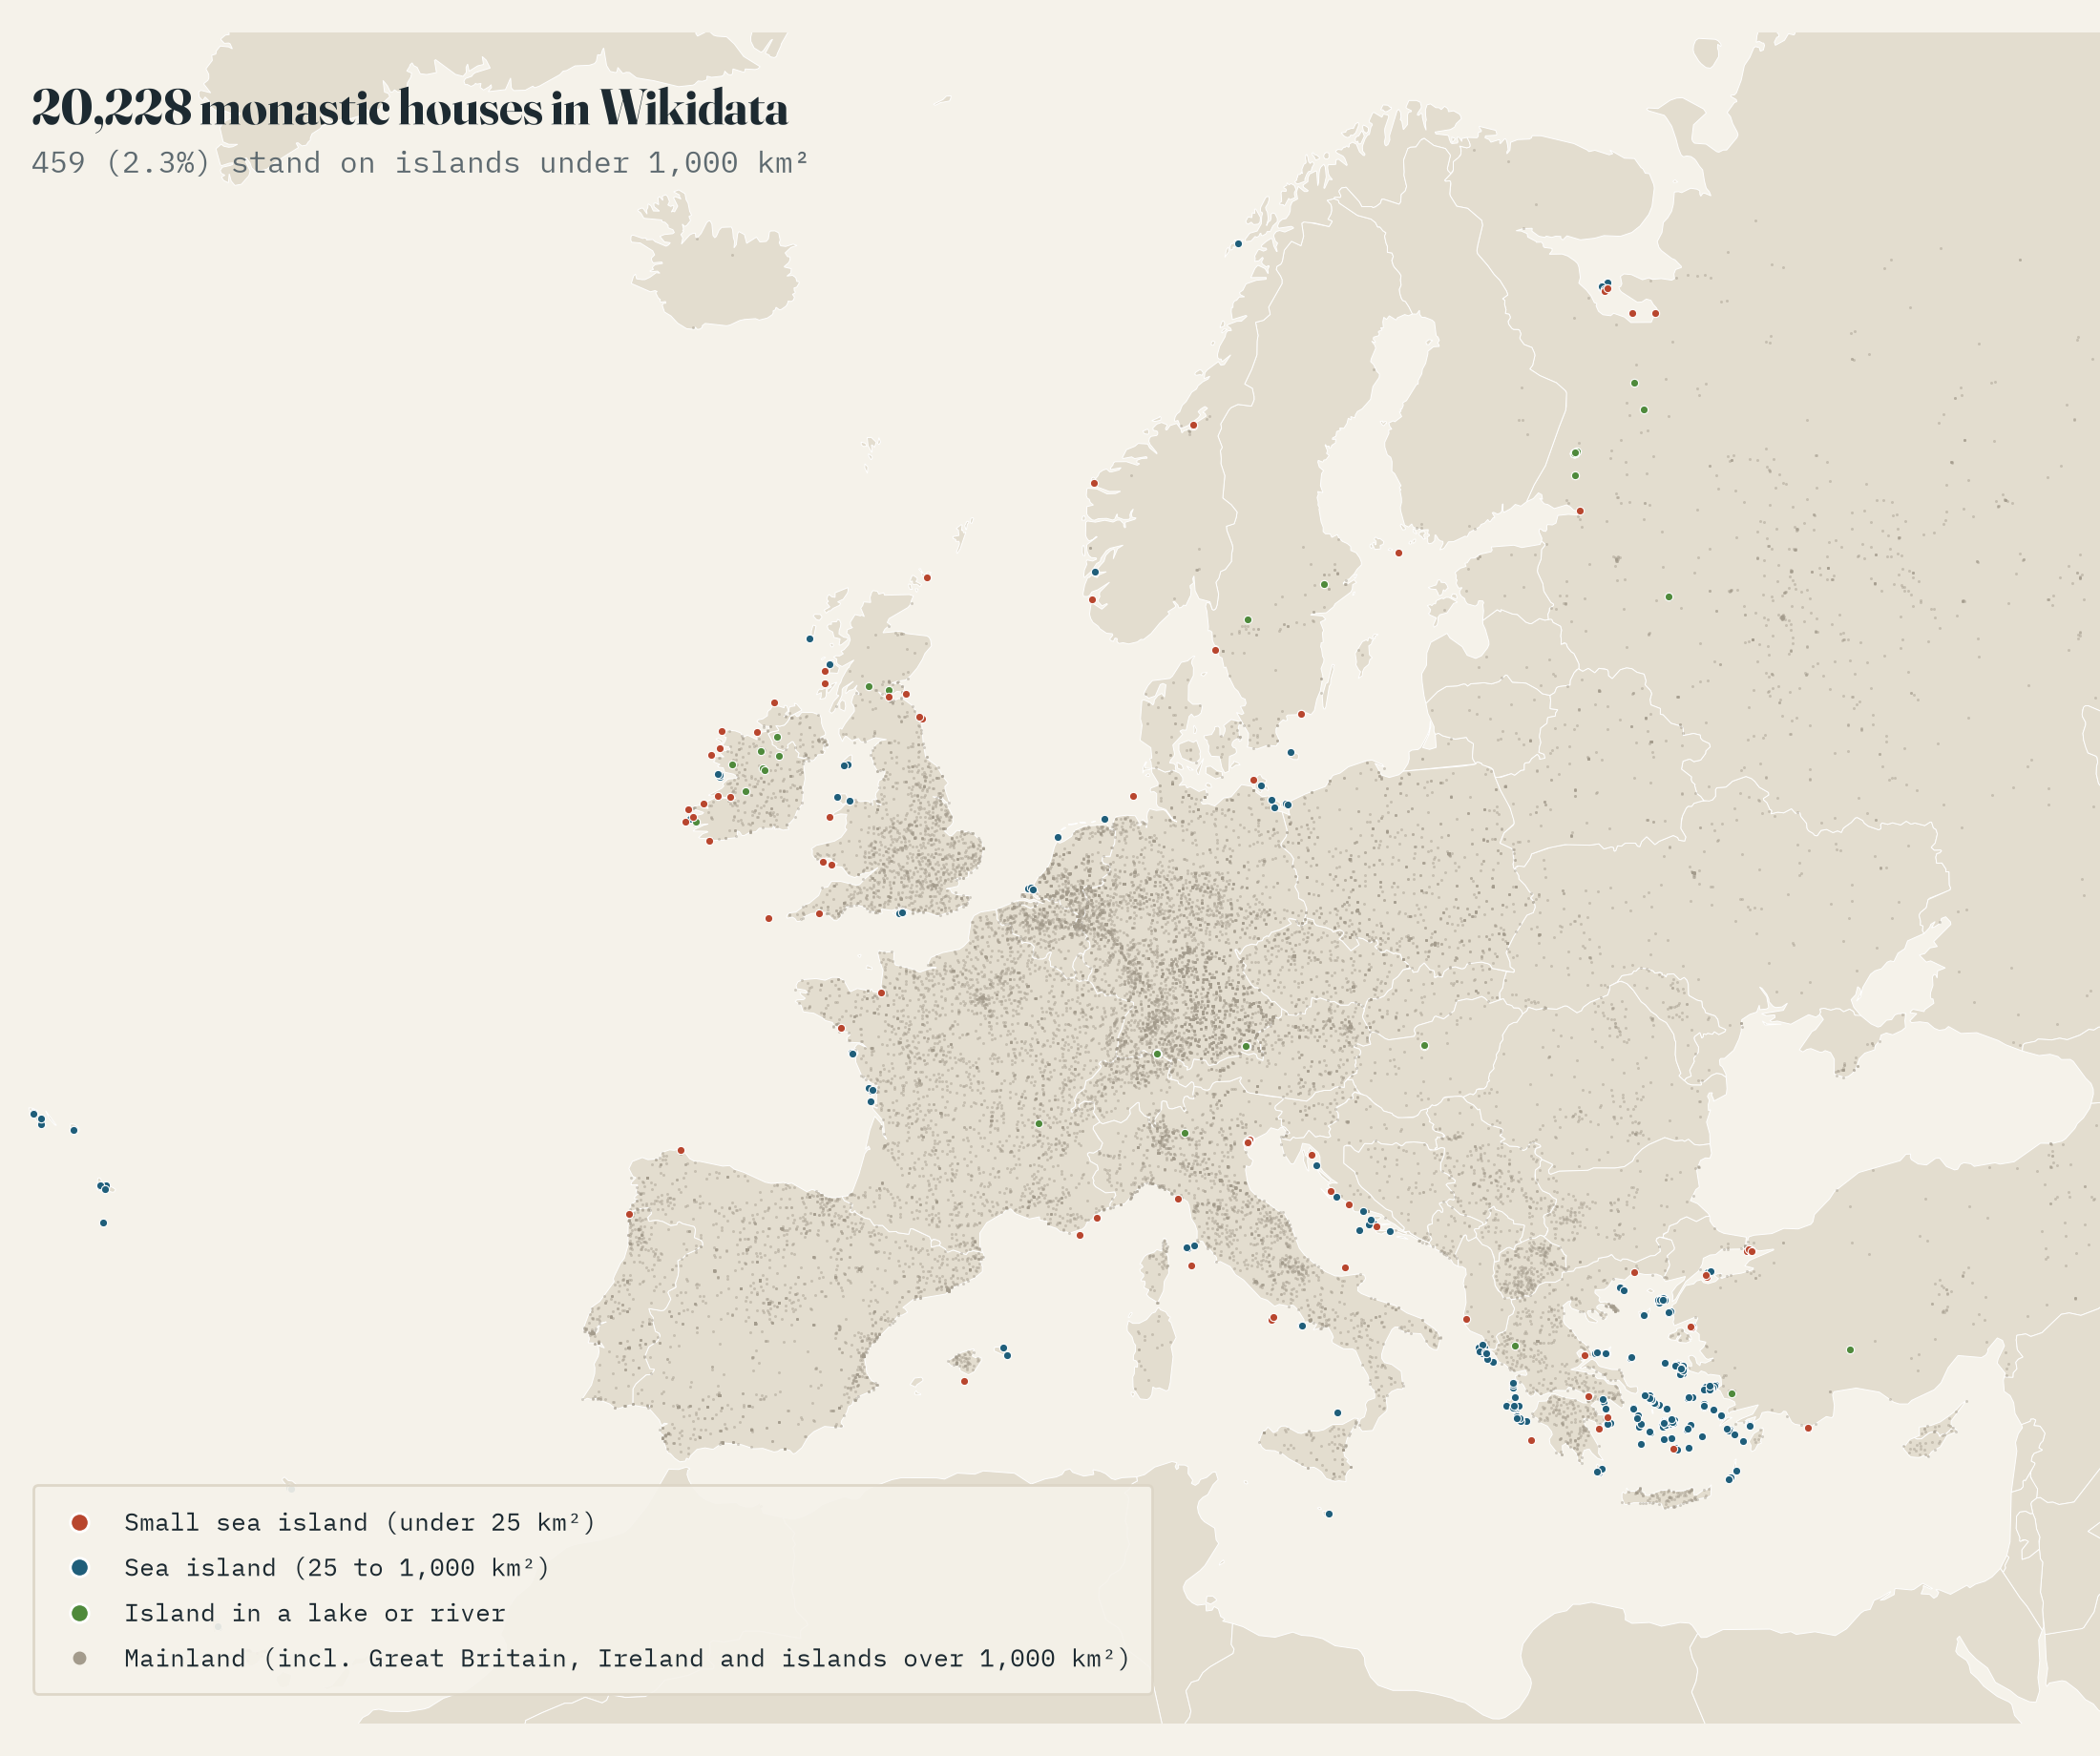
\includegraphics[width=\textwidth]{f_map_europe.png}
\caption{Monastic houses in Wikidata, by setting. Grey: mainland, including Great Britain, Ireland and islands over 1,000 km$^2$.}\label{fig:map}\end{figure}

\subsection{By date of foundation}
The share of island houses is highest among the earliest foundations (Figure~\ref{fig:per}, Table~\ref{tab:reg}). Of 255 houses dated before 800, 11 are on islands (4.3\%, interval 2.4 to 7.6\%): Lérins and Cabrera in the western Mediterranean; Bardsey, Caldey, Iona, Douglas on the Isle of Man and Mont-Saint-Michel on the Atlantic side; and Reichenau, Herrenchiemsee, Frauenchiemsee and the Île Barbe in lakes and rivers. The share is 1.1\% for houses founded from 1100 to 1299 (24 of 2,220), the period of the Cistercians, the regular canons and the friars, and 1.2\% after 1300. The century series (Figure~\ref{fig:cent}) shows the same pattern, with very few dated houses before the 900s.

On the Atlantic Celtic edge, 3 of the 28 houses dated before 1100 are on islands (Bardsey, Caldey and Iona; 10.7\%), against 5 of 3,230 houses founded in France and Central Europe from 1100 (0.2\%). The early Atlantic foundations therefore chose islands far more often than the later Continental ones, although the Atlantic estimate rests on very few dated houses and its interval runs from 3.7 to 27.2\%. Including undated houses, the Atlantic edge has 6.3\% of houses on islands and France and Central Europe 0.3\%.

Reading years ending in 00 as the middle of the century they begin rather than end moves the all-Europe shares only slightly (4.6\%, 1.8\%, 1.0\% and 1.3\% for the four periods) and leaves the early Atlantic share at 10.7\%. Restricting to exactly dated houses gives 5.2\% before 800 and 1.0\% for 1100 to 1299. Counting only small islands under 25 km$^2$, the share is 2.4\% before 800 and 0.2\% after 1300.

\begin{figure}[tbp]\centering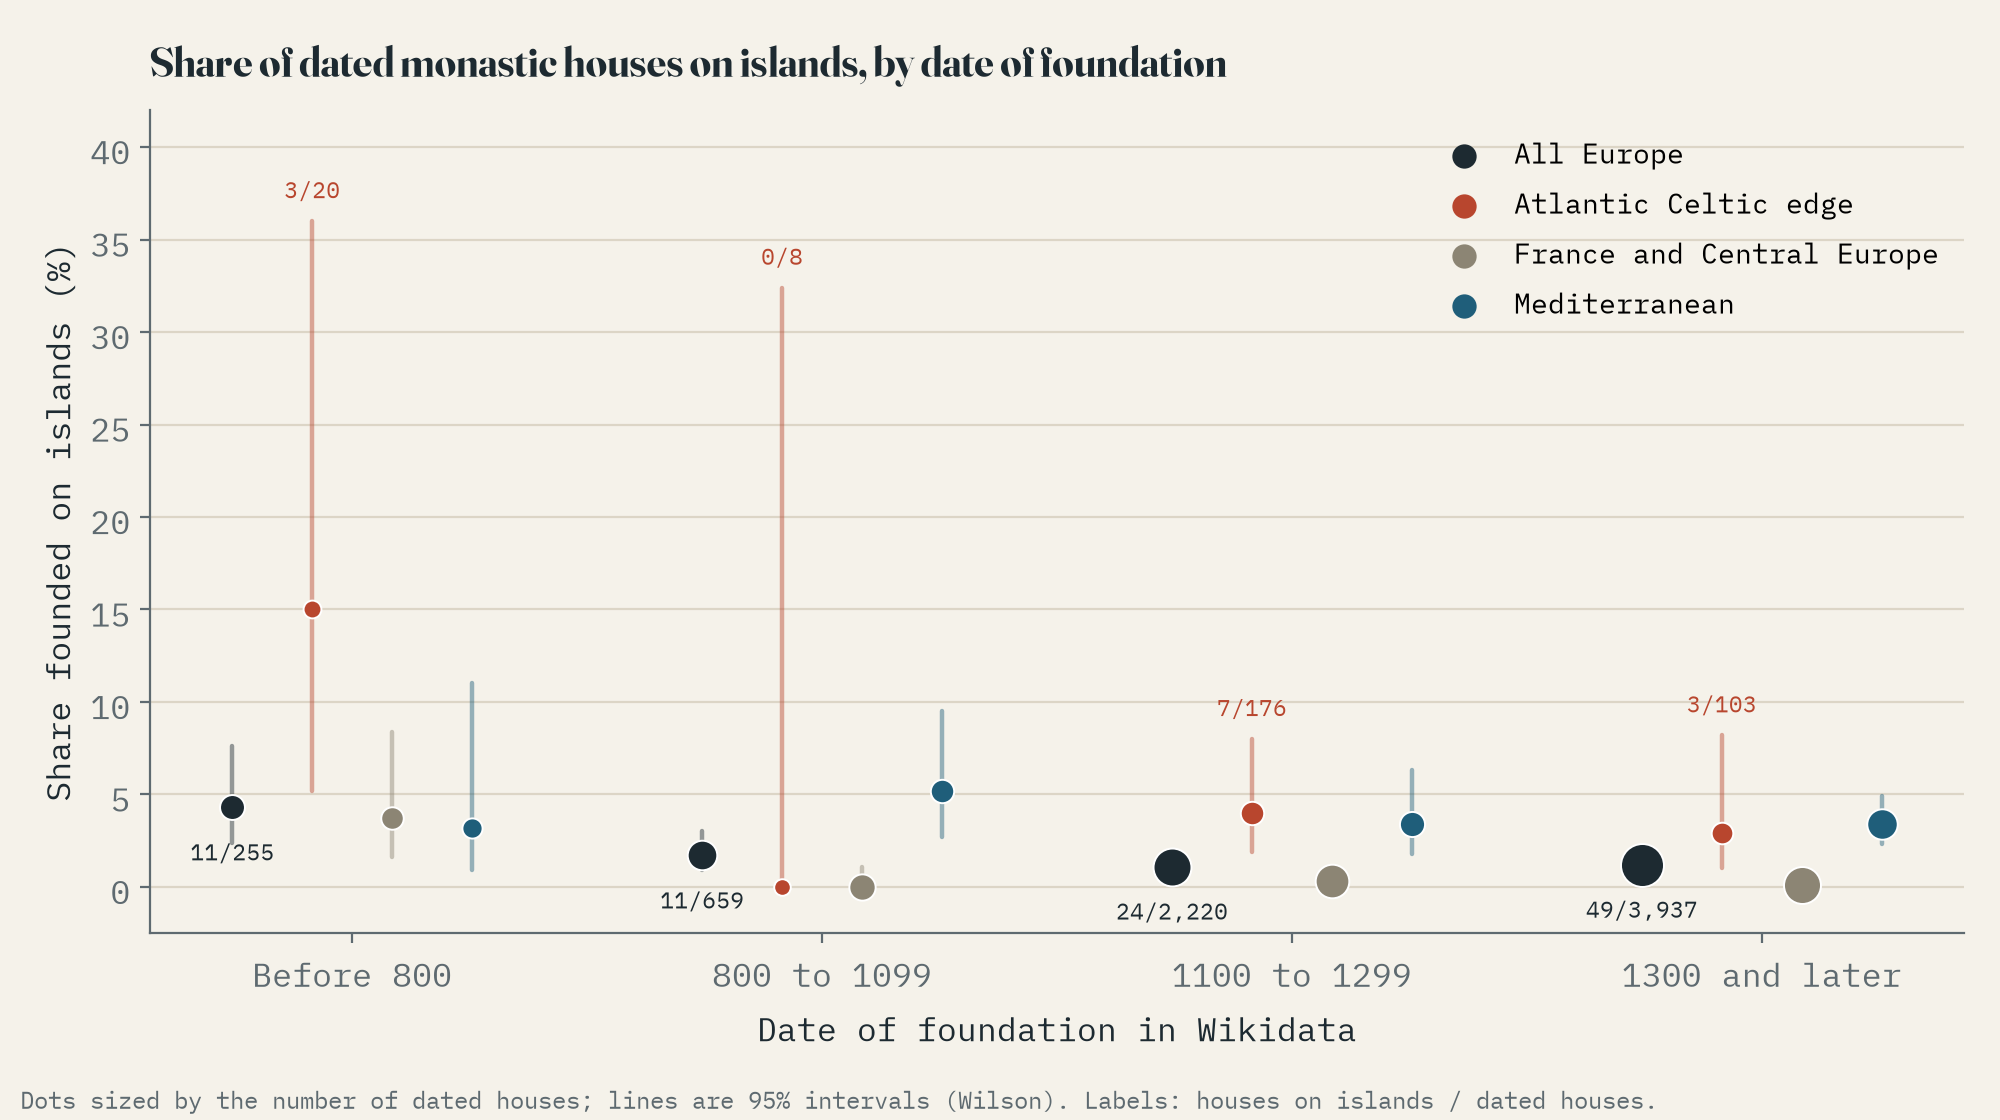
\includegraphics[width=\textwidth]{f_periods.png}
\caption{Share of dated houses on islands by period of foundation, for all Europe and three groups of regions, with Wilson 95\% intervals.}\label{fig:per}\end{figure}

\begin{figure}[tbp]\centering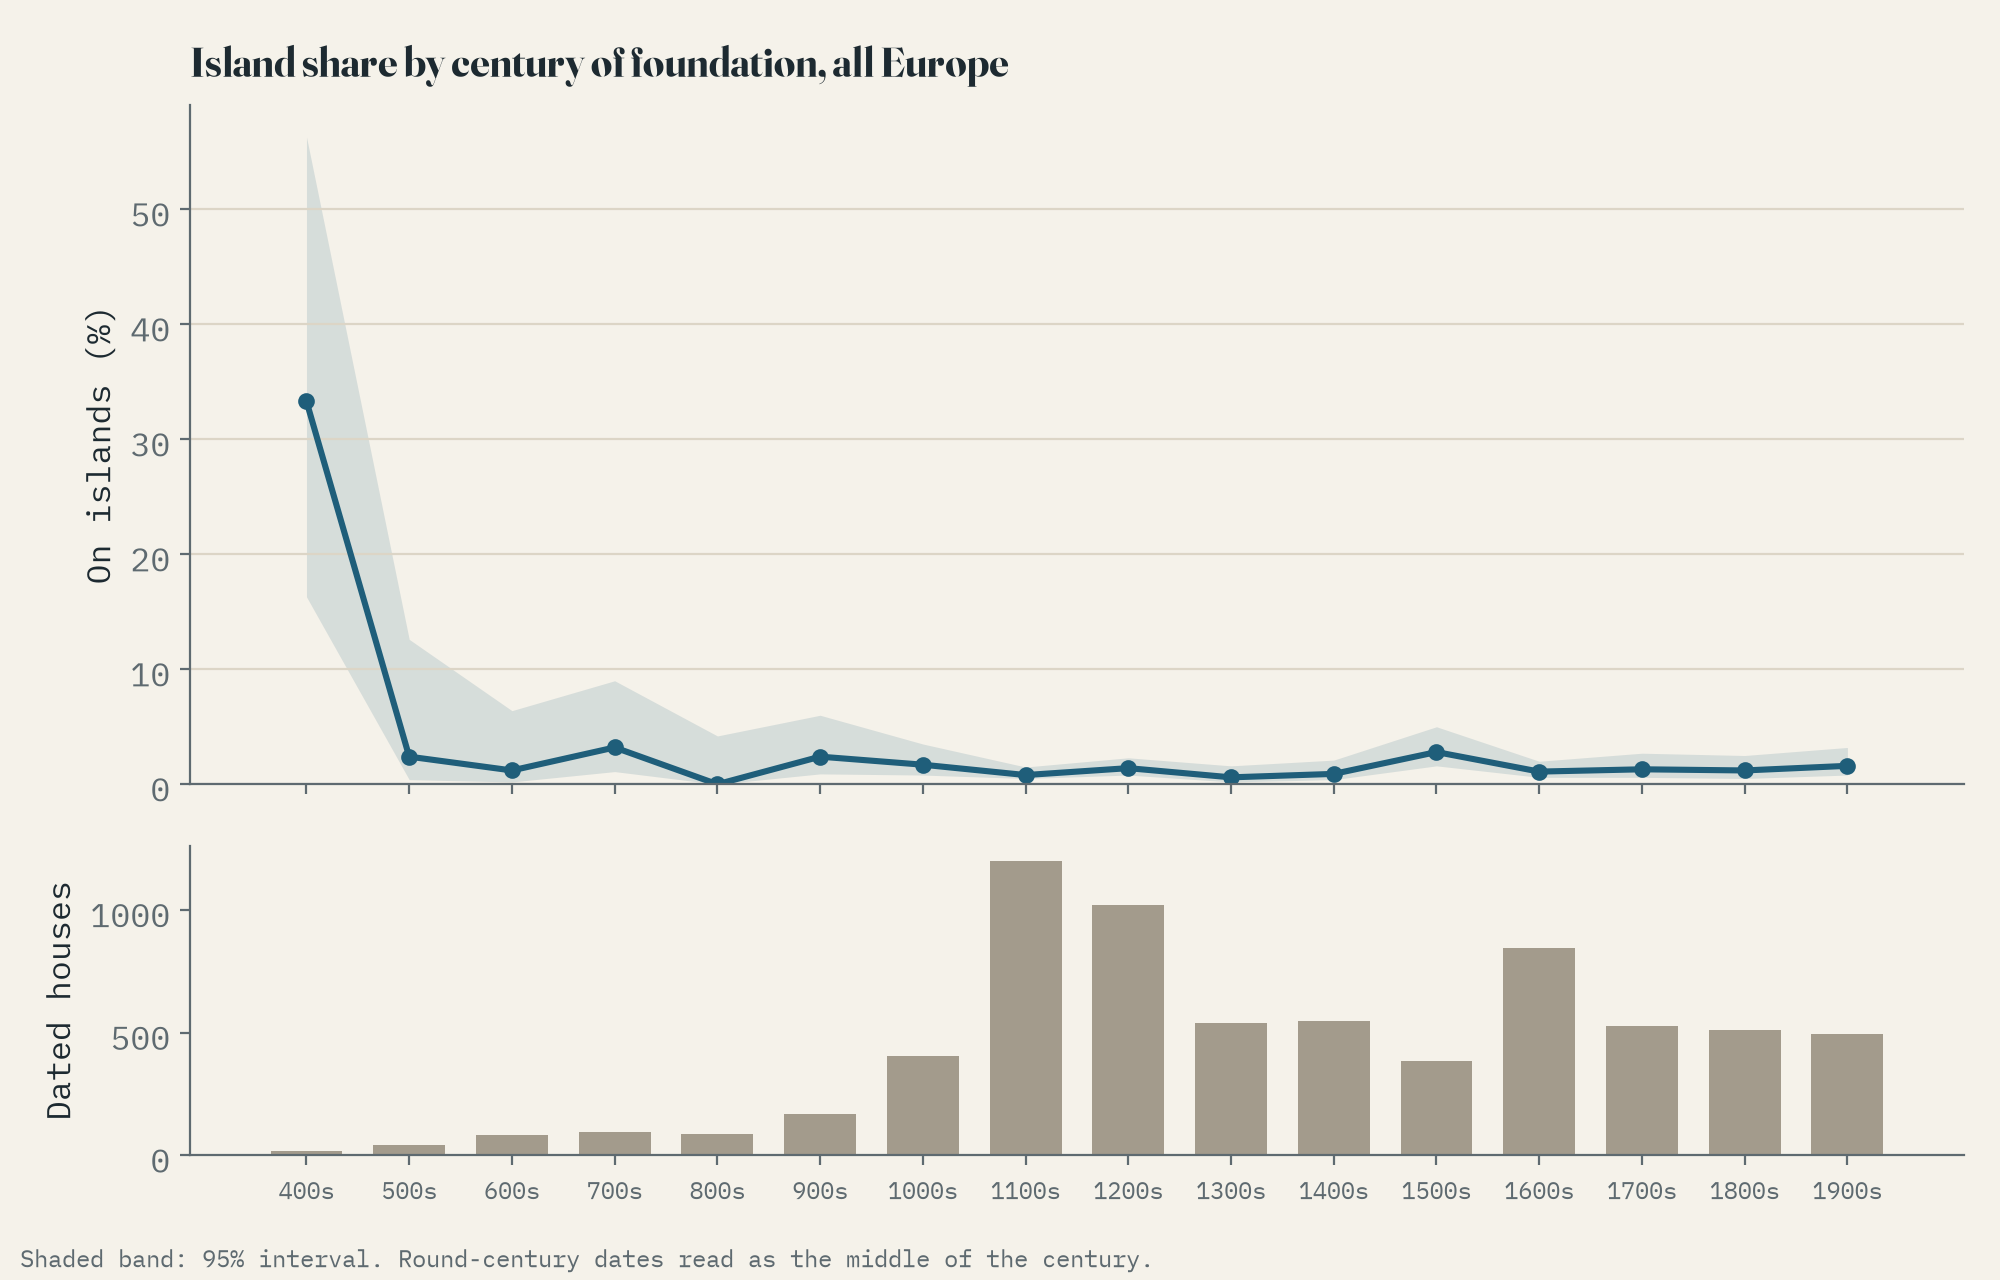
\includegraphics[width=\textwidth]{f_century.png}
\caption{Share of dated houses on islands by century of foundation, all Europe, with the number of dated houses per century.}\label{fig:cent}\end{figure}

\subsection{By region}
Counting all houses, dated or not (Figure~\ref{fig:reg}), the highest island shares are in Wales (13.0\%, 7 of 54) and Scotland (12.4\%, 11 of 89), followed by the Mediterranean (7.7\%) and Ireland (7.5\%). The Mediterranean has by far the most island houses (304), 83\% of them on Greek and Turkish islands, mostly Orthodox monasteries and mostly undated. Brittany (0.8\%) and Galicia (1.0\%) have few island houses in this record despite their many coastal islands and their early saints. France and Central Europe have 0.3\%, and 15 of their 34 island houses are on lake or river islands. Iceland and the Faroes have only 3 houses in the data.

By kind of house, those Wikidata calls simply monasteries are most often on islands (3.0\%), reflecting the Orthodox monasteries of the Aegean; abbeys (1.0\%), priories (0.9\%) and convents (0.8\%) much less. Hermitages, despite the eremitic ideal, are on islands in 1.5\% of cases, because the class is dominated by Italian and Spanish hermitages, most of them inland.

\begin{table}[tbp]\centering\footnotesize\caption{Houses on islands / houses, by region and period of foundation; the last two columns include undated houses.}\label{tab:reg}\setlength{\tabcolsep}{4pt}\begin{tabular}{>{\raggedright\arraybackslash}p{4.4cm}rrrrrr}\toprule Region & Before 800 & 800 to 1099 & 1100 to 1299 & 1300 and later & All & \%\\\midrule
Ireland & 0/14 & 0/2 & 2/78 & 0/70 & 24/321 & 7.5\\
Scotland & 1/2 &  & 4/40 & 1/6 & 11/89 & 12.4\\
Wales & 2/2 & 0/1 & 1/23 & 1/3 & 7/54 & 13.0\\
England, Man and the Channel Islands & 1/29 & 1/69 & 2/320 & 1/46 & 11/1,202 & 0.9\\
Brittany & 0/1 & 0/2 & 0/22 & 1/15 & 1/133 & 0.8\\
France (rest) & 2/54 & 0/94 & 2/322 & 0/195 & 8/2,385 & 0.3\\
Galicia & 0/1 & 0/3 & 0/13 & 0/9 & 1/100 & 1.0\\
Iberia (rest) & 0/7 & 0/26 & 0/84 & 3/250 & 23/1,558 & 1.5\\
Iceland and the Faroes &  &  & 0/2 &  & 0/3 & 0.0\\
Scandinavia and the Baltic &  & 1/7 & 2/48 & 1/43 & 14/213 & 6.6\\
Central Europe and the Low Countries & 3/81 & 0/257 & 2/933 & 1/1,780 & 26/8,346 & 0.3\\
Mediterranean & 2/62 & 9/174 & 9/268 & 26/769 & 304/3,928 & 7.7\\
Eastern Europe and the Balkans & 0/2 & 0/24 & 0/67 & 14/751 & 29/1,896 & 1.5\\
\bottomrule\end{tabular}\end{table}

\begin{figure}[tbp]\centering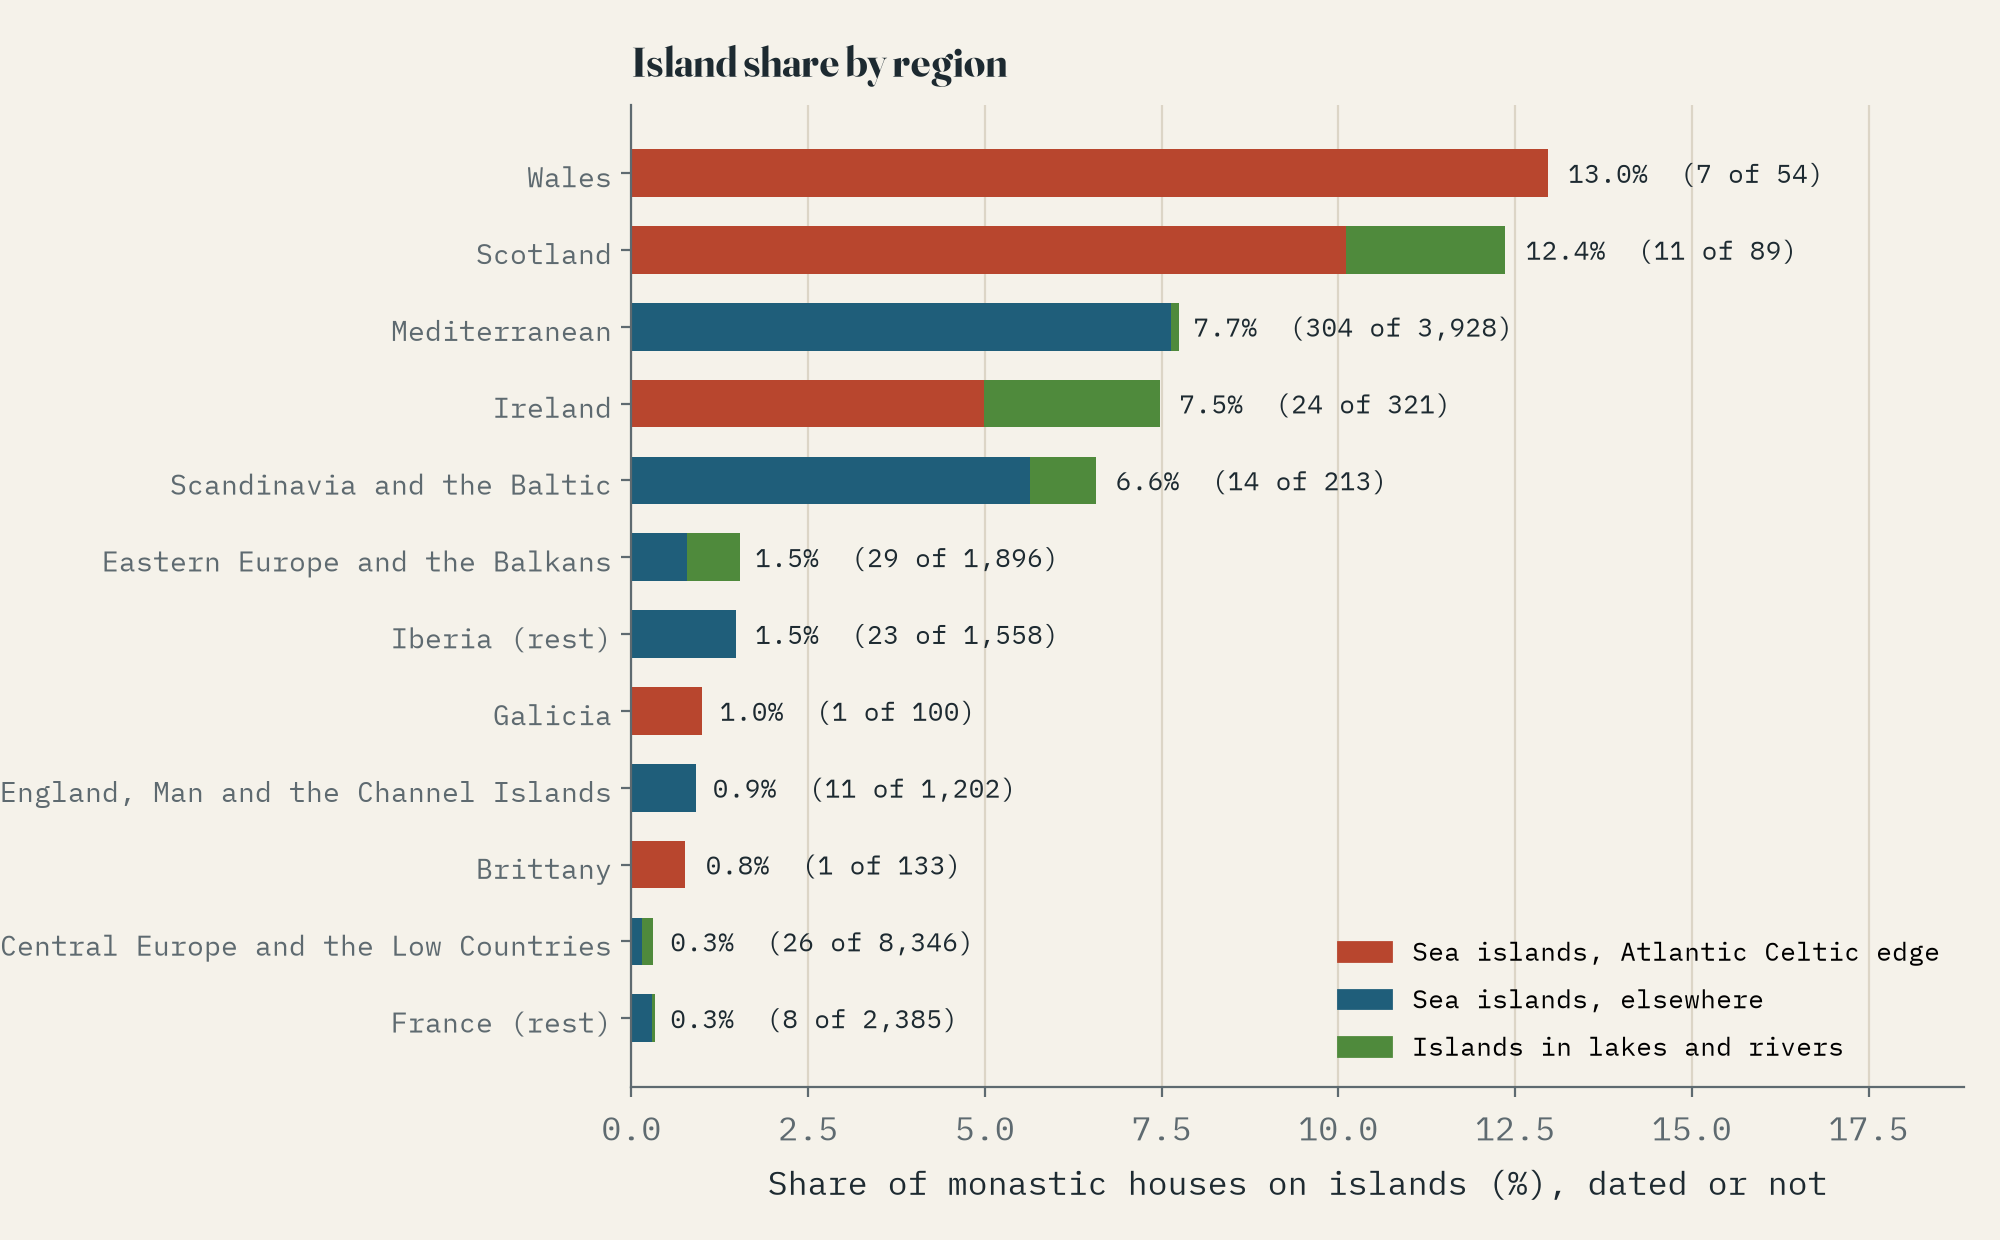
\includegraphics[width=.92\textwidth]{f_regions.png}
\caption{Share of houses on islands by region (regions with at least 20 houses), all houses dated or not.}\label{fig:reg}\end{figure}

\begin{figure}[tbp]\centering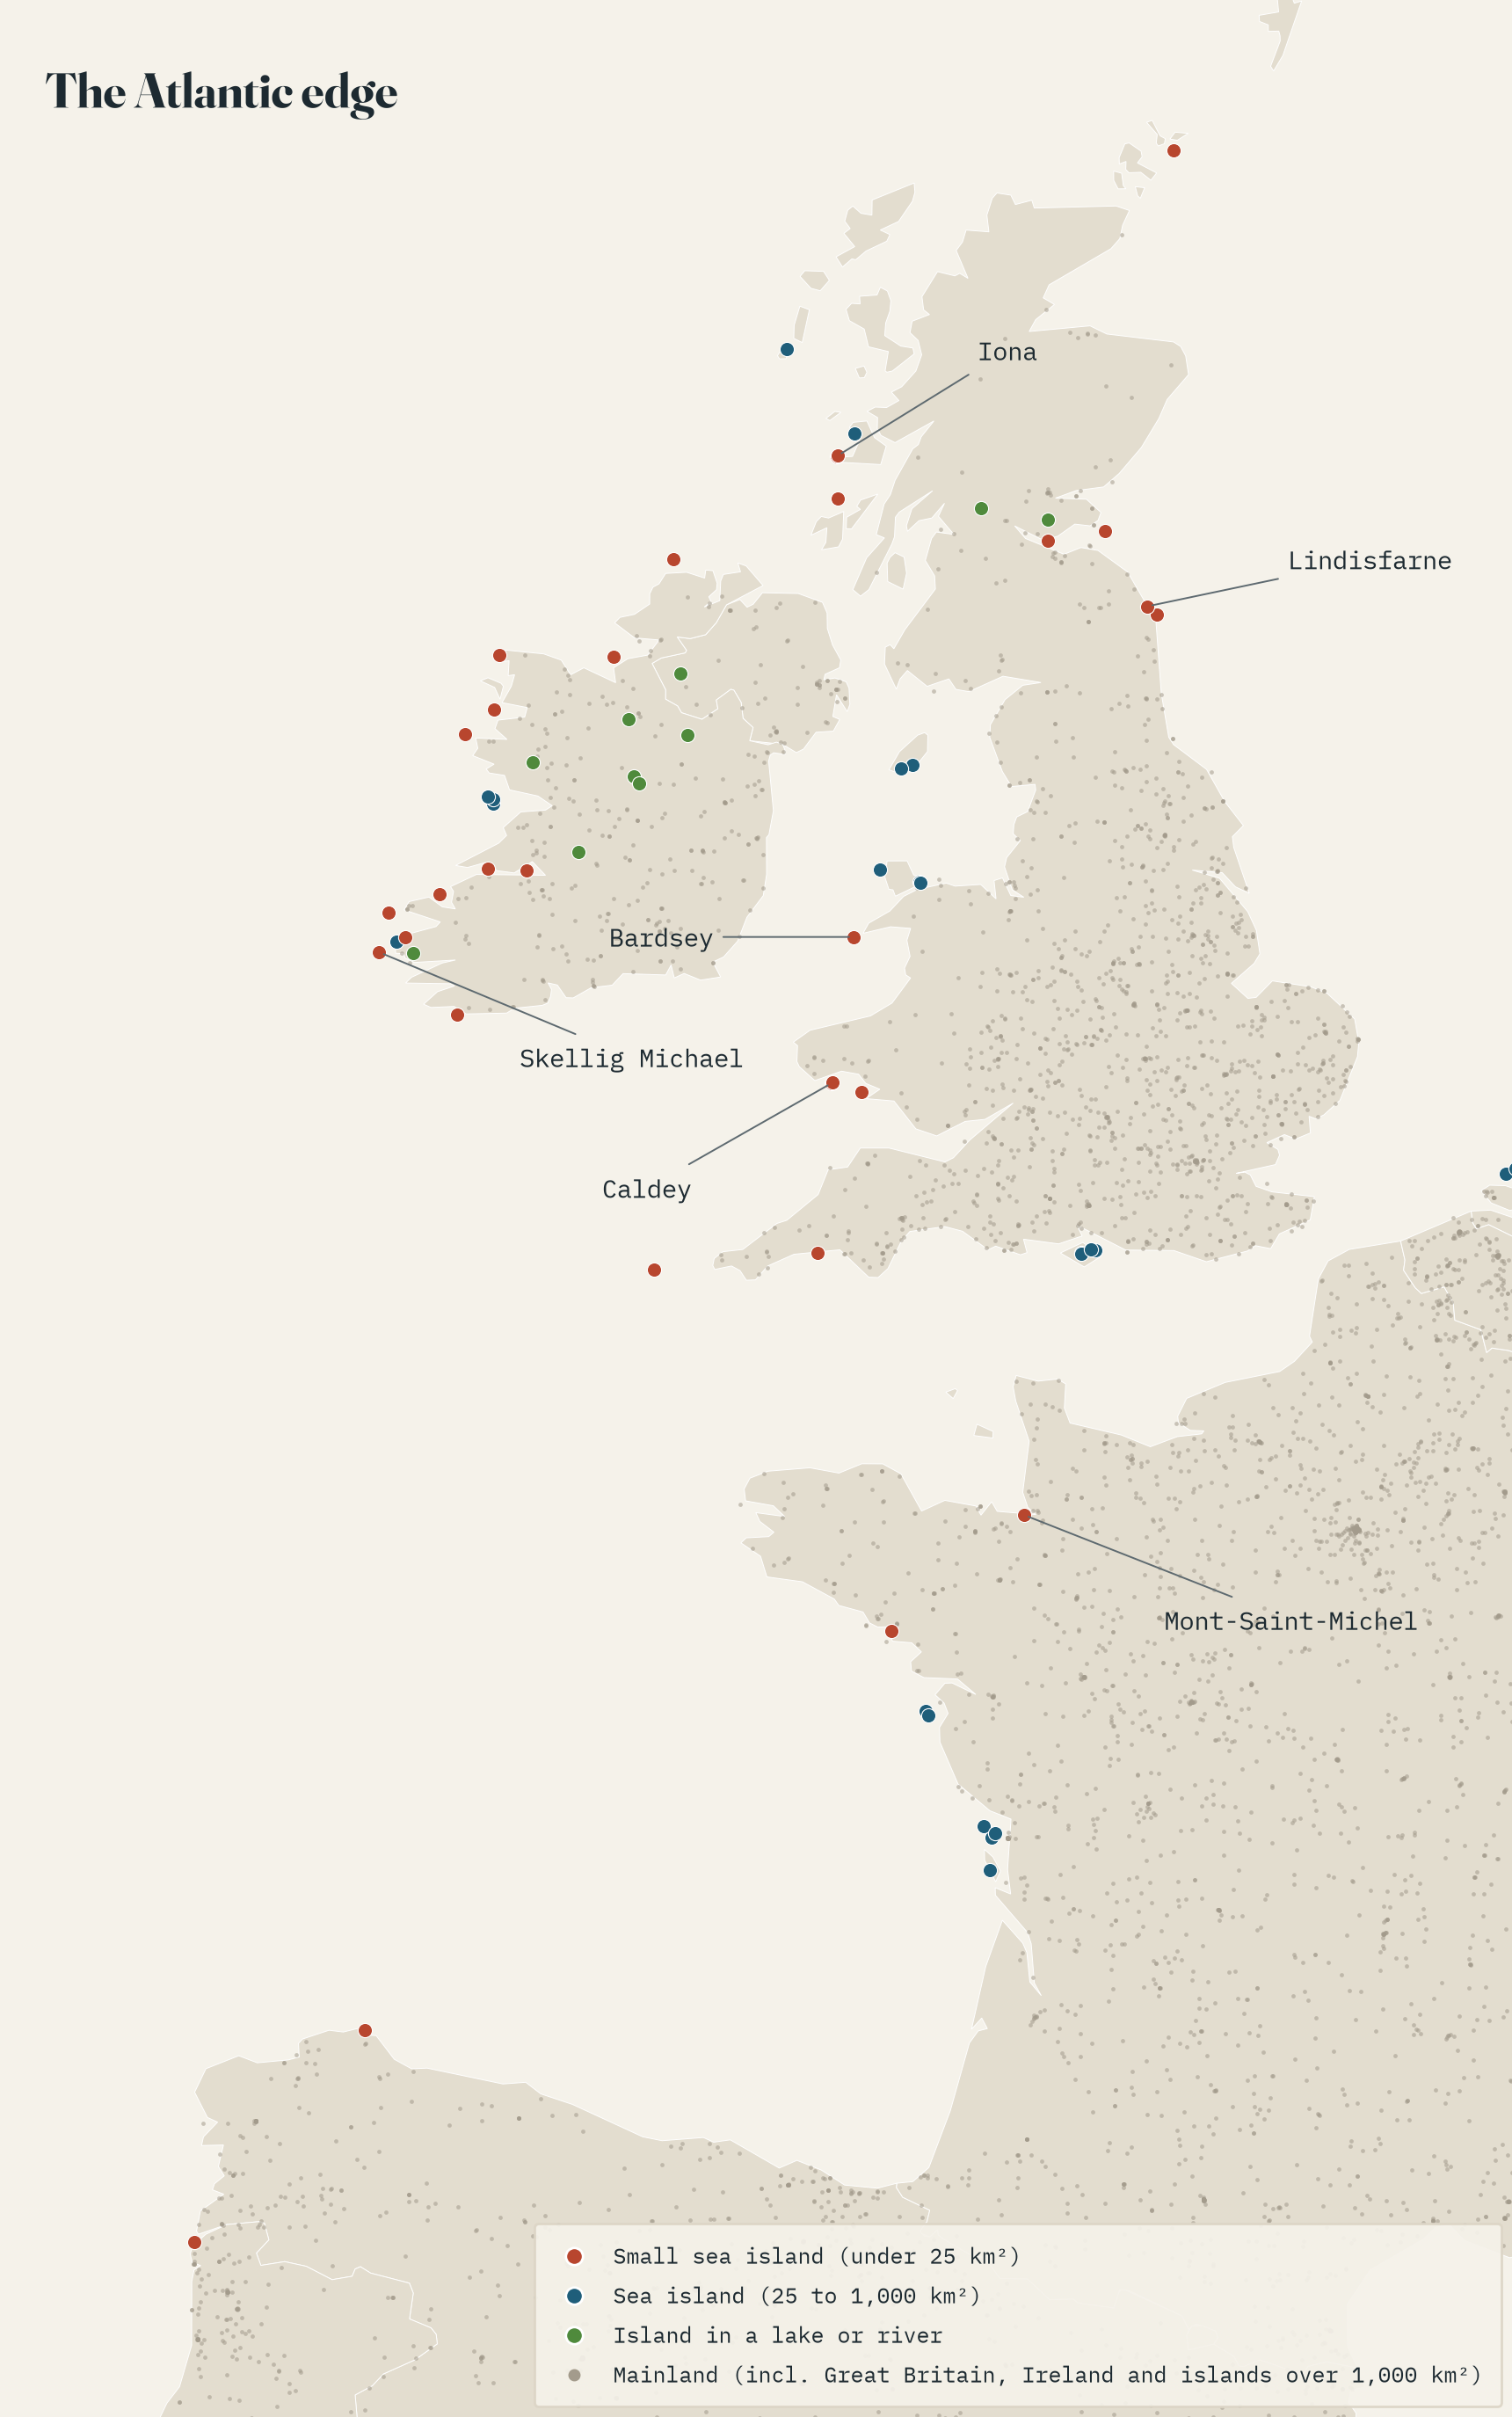
\includegraphics[width=.9\textwidth]{f_map_atlantic.png}
\caption{The Atlantic edge: houses by setting, with five famous island houses named.}\label{fig:atl}\end{figure}

\subsection{Distance from the mainland}
Half of the sea-island houses are within 24.4 km of the mainland, and 72 are more than 100 km out (Figure~\ref{fig:far}). The furthest are the convents of the Azores, founded after Portuguese settlement in the fifteenth century: the Convent of Carmo at Horta on Faial is 1,656 km from the mainland. Madeira (667 km), La Palma in the Canaries (444 km) and Malta (249 km) follow. Of houses founded before 1300, the furthest is the Hozoviotissa monastery on Amorgos (121 km). On the larger islands counted as mainland, Iceland's Þingeyrar (1133) is 1,100 km from the nearest mainland coast. The Celtic holy islands are close in by comparison: Skellig Michael is 12.3 km out, Iona 38.1 km, and the furthest in Britain and Ireland is Cille Bharra on Barra (81.0 km). On lakes, the Valaam sketes are up to 24.6 km from the shore of Ladoga.

\begin{figure}[tbp]\centering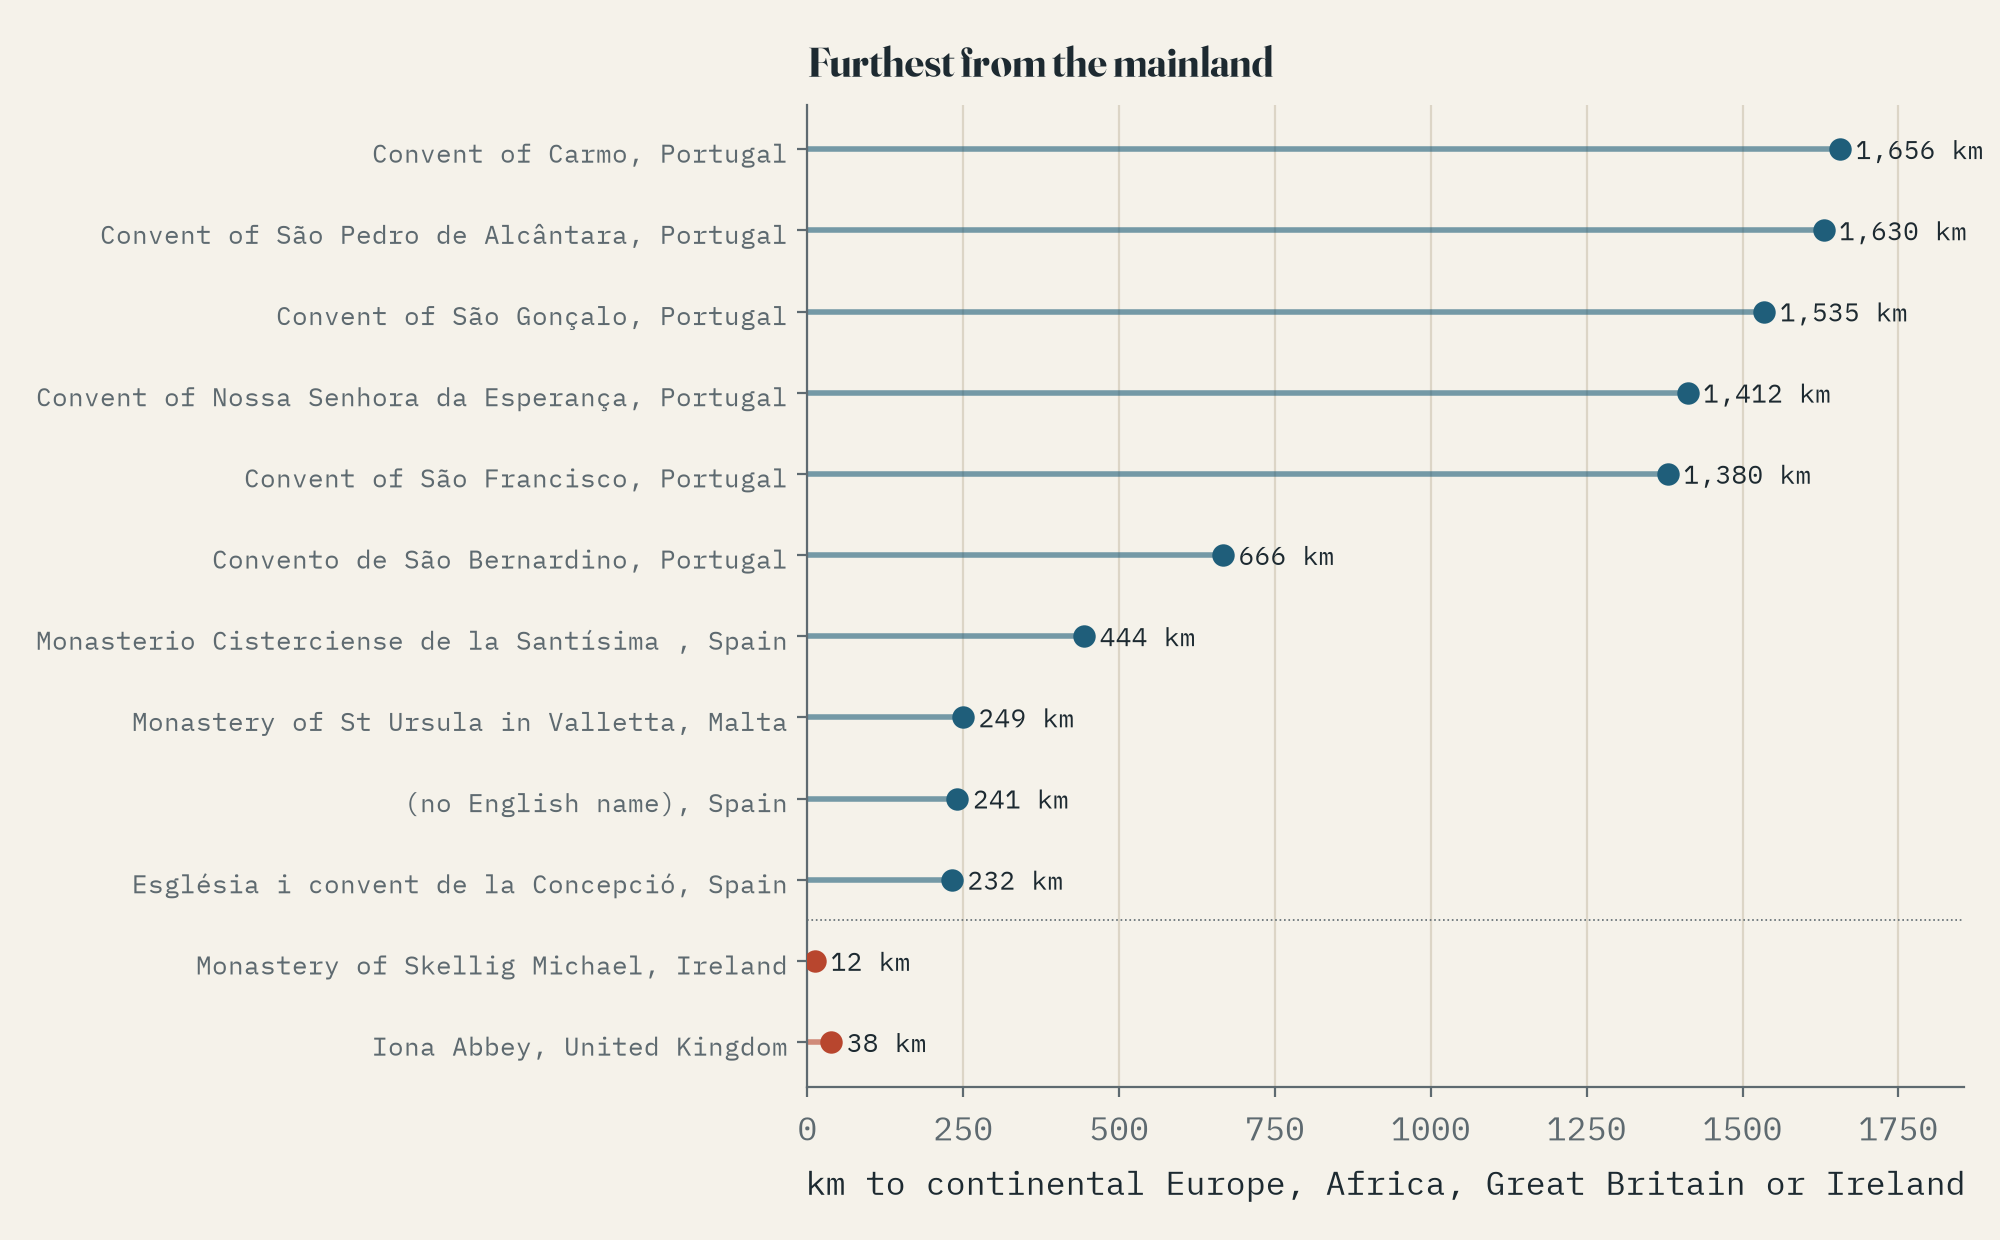
\includegraphics[width=\textwidth]{f_far.png}
\caption{Island houses furthest from continental Europe, Africa, Great Britain or Ireland (one per island), with Skellig Michael and Iona.}\label{fig:far}\end{figure}

\subsection{Dissolution and abandonment}
2,944 houses (14.6\%) have a date of dissolution or abandonment (Figure~\ref{fig:dis}); another 821 are classed as ruins or former houses without a date. The dates fall in waves: 614 in England and Wales from 1536 to 1541 (96\% of all dated closures there), 36 of 41 in Ireland from 1536 to 1600, 245 in France from 1789 to 1795, 492 in the German lands from 1802 to 1811 and 71 in Spain from 1835 to 1837. The Reformation century and the revolutionary era together hold 73\% of all dated closures.

The Viking age, which fell first on island monasteries, is almost invisible: 18 closures are dated between 793 and 1066, all on the mainland. The record describes houses as they were last constituted: Lindisfarne Priory is the Benedictine cell refounded in 1093 and Bardsey Abbey's dissolution date is 1537. Island houses carry a closure date less often than mainland ones (4.4\% against 14.8\%; 9.7\% outside Greece and Turkey), and where they do, the median year is 1,541 against 1,602.

\begin{figure}[tbp]\centering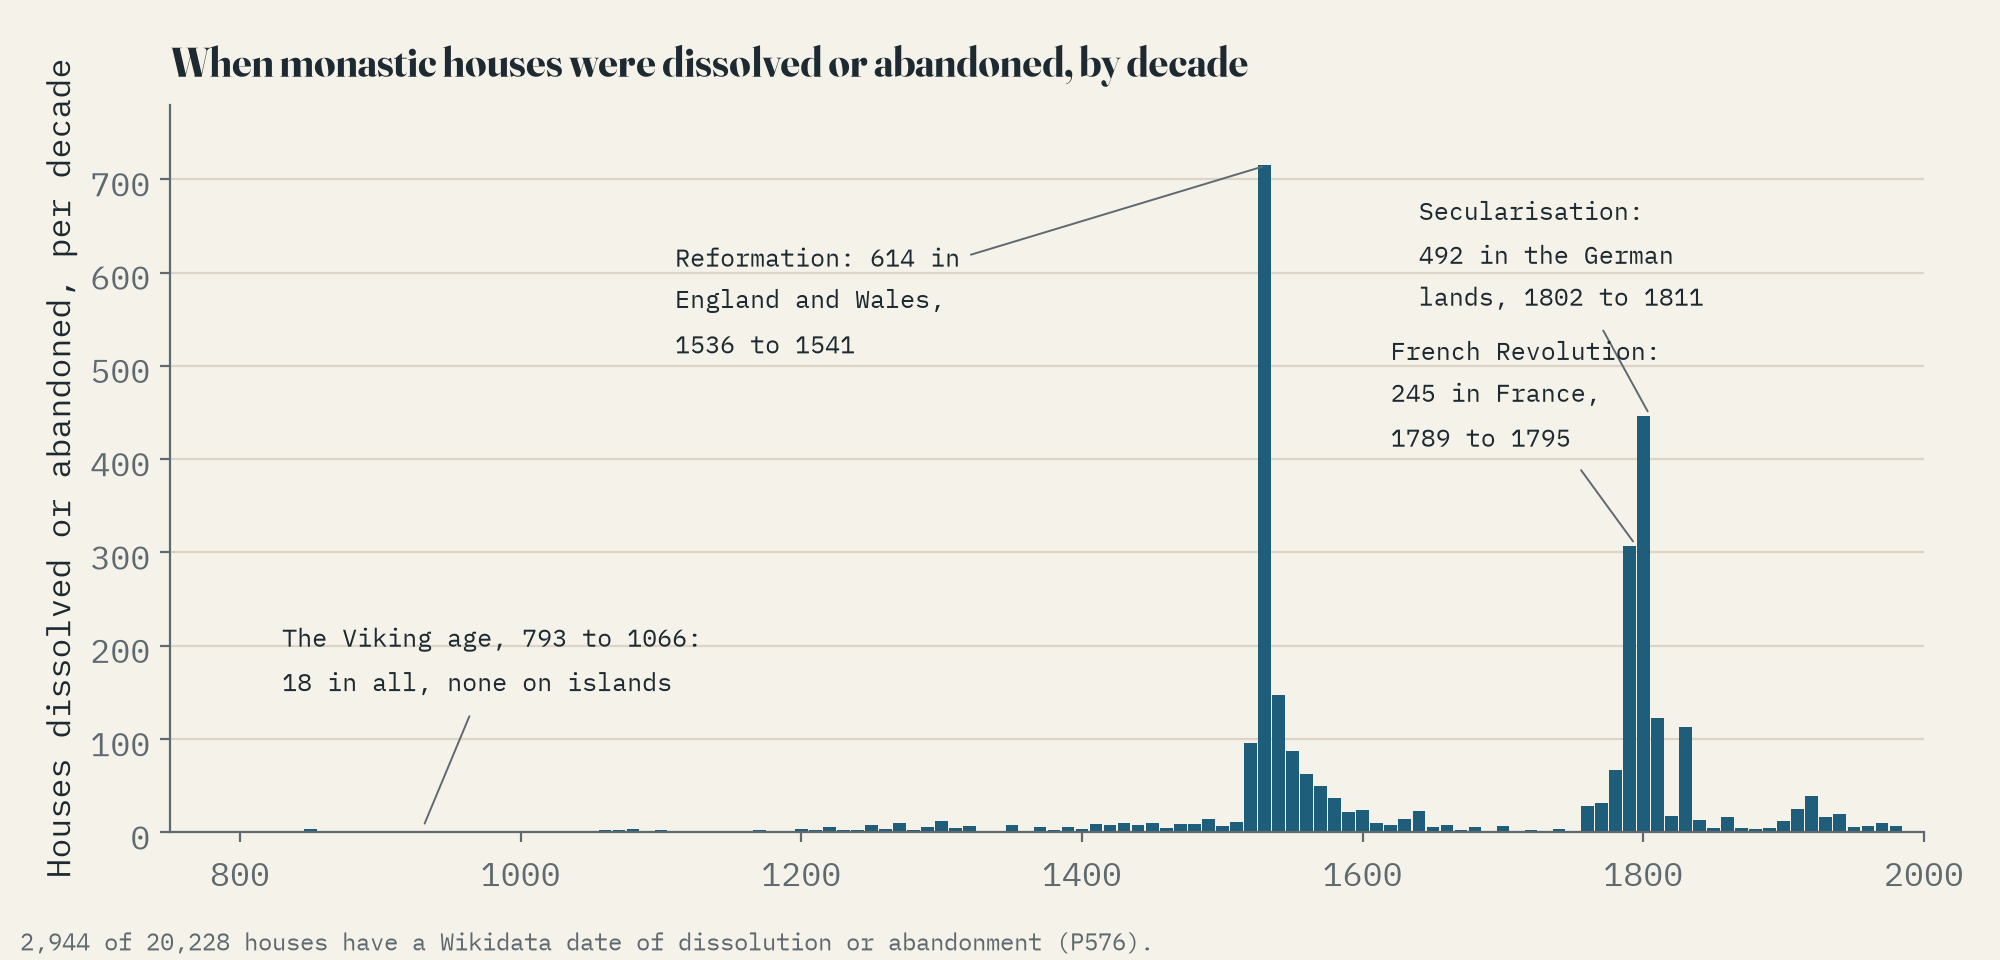
\includegraphics[width=\textwidth]{f_dissolution.png}
\caption{Houses dissolved or abandoned, by decade of the Wikidata date.}\label{fig:dis}\end{figure}

\subsection{Coverage}
The record is uneven (Figure~\ref{fig:cov}). Germany holds 24.1\% of houses; houses per million people range from 132 in North Macedonia and 59 in Germany to 1.8 in Finland among countries of over two million people. Ireland has 321 houses in the data (north and south), a small fraction of its recorded early ecclesiastical sites, many of which are classed in Wikidata as churches, archaeological sites or ecclesiastical sites rather than monasteries. Only 35\% of houses have a foundation date, from under a third in France, Galicia and Iberia to about half in Ireland, Scotland and Wales, and Skellig Michael is among those without one. Half of all houses have 1 Wikipedia article or fewer; 29.4\% have none.

\begin{figure}[tbp]\centering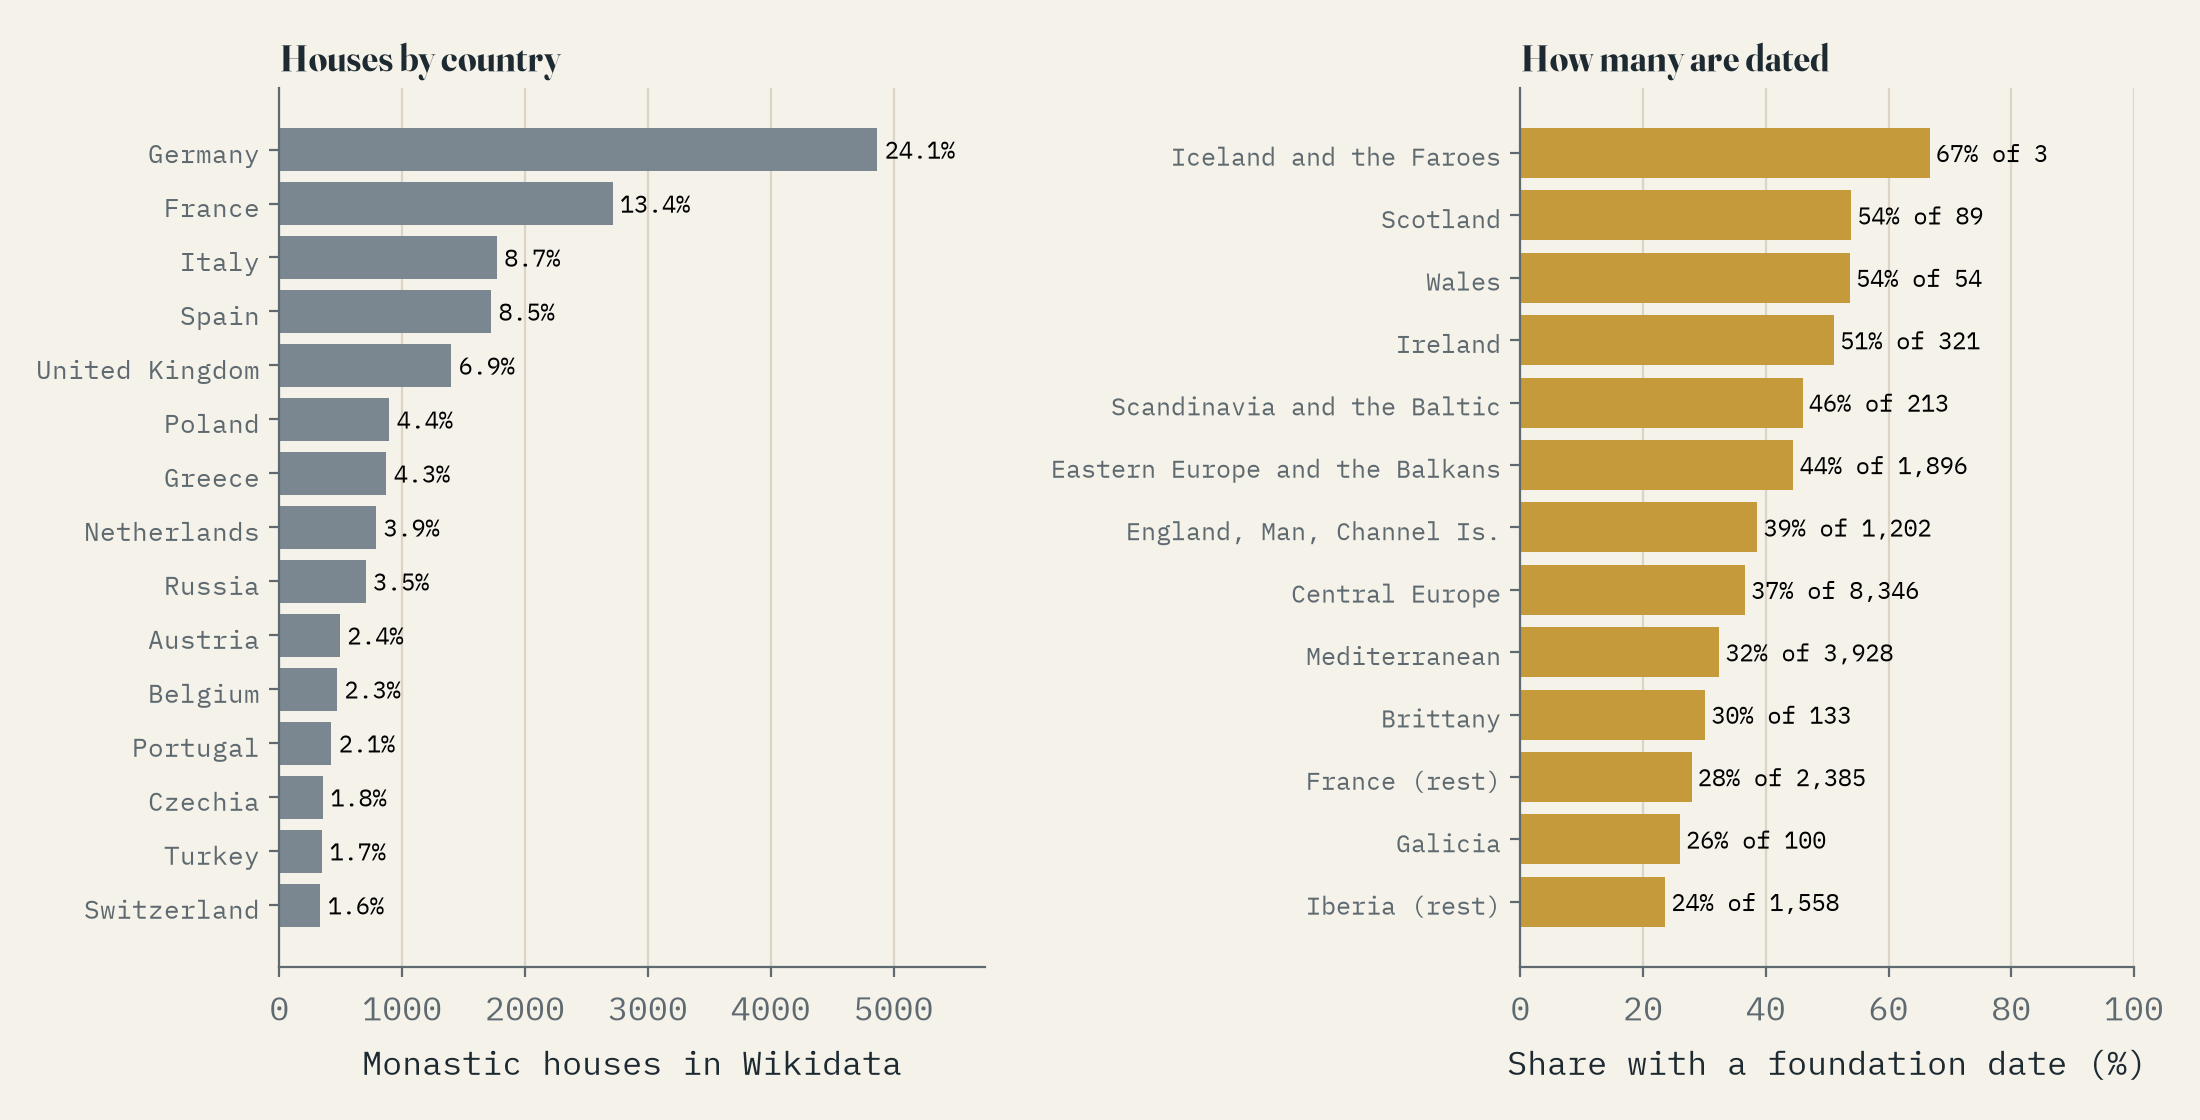
\includegraphics[width=\textwidth]{f_coverage.png}
\caption{Houses by country (top 15) and the share with a foundation date by region.}\label{fig:cov}\end{figure}

\section{Discussion}
The data support the familiar story, with qualifications. Early foundations, before 800, were several times more likely to be on islands than those of the high and late Middle Ages, and the contrast between the early Atlantic edge and the later Continental foundations is large. The island monastery was a feature of a particular moment and a particular coast, and of the late antique Mediterranean that inspired it, rather than of monasticism in general. After 1100 new orders sought other solitudes: the Cistercians' remote valleys, the Carthusians' mountains, and then the friars' towns.

The Orthodox world offers a contrast. The Aegean islands hold more monastic houses than anywhere else, and Valaam, Konevets and Solovetsky took the island ideal to the lakes and seas of the Russian north in the fourteenth and fifteenth centuries. Here the island monastery was a lasting tradition, not an early phase, and many houses are still active, which is one reason why island houses are less often recorded as dissolved.

The dissolution dates show how far the record reflects the institutions that survived longest. The Viking raids that ended or interrupted the early island communities are absent, while the Dissolution of the Monasteries, the French Revolution and the German secularisations stand out sharply, because the houses then closed were well documented institutions whose ends were recorded.

\section{Limitations}
First, coverage: Wikidata's monastery records depend on which national lists have been loaded and how early sites are classified, and the early Atlantic sample is small. Second, dates: inception may record a refoundation, precision is lost in the extract, and only a third of houses are dated. Third, geography: present-day shorelines are used, so islands since joined to the land (and land since lost to the sea) are classified as they are now; small lake and river islands are undercounted despite the hand checks; the 1,000 km$^2$ threshold is a choice, and other choices are reported. Fourth, points: a few coordinates are imprecise or refer to a later site of a community. Fifth, the study counts records and cannot speak to motives.

\section{Conclusion}
Of the monastic houses that Wikidata places in Europe, about one in forty stands on an island. The share was highest among the earliest foundations and on the Atlantic edge, and the Aegean holds the most island houses of all. The analysis is open and reproducible, and its gaps point to where the record could be improved: dates, early Irish sites, and the papar of the North Atlantic.

\section*{Data and code availability}
The interactive map is at \url{https://maps.tristanhotham.com/holy-islands/}. Data and code are at \url{https://github.com/Tristan-Hotham/holy-islands} and archived with this paper at \url{https://doi.org/10.5281/zenodo.23844515}. Wikidata content is CC0; island outlines derived from GSHHG are LGPL-3.0; the derived data and text are released under CC BY 4.0 and the code under the MIT licence.

\section*{AI statement}
I wrote the text, with drafting and editing assistance from Claude (Anthropic), which also helped prepare the analysis code. I reviewed and checked all text and results.

\begin{thebibliography}{9}
\bibitem[Bast and Buchhold(2017)]{qlever} Bast, H. and Buchhold, B. (2017) QLever: a query engine for efficient SPARQL+text search. \emph{Proceedings of the 2017 ACM Conference on Information and Knowledge Management}, 647 to 656.
\bibitem[Dicuil(825)]{dicuil} Dicuil (c. 825) \emph{Liber de mensura orbis terrae}. Ed. J. J. Tierney (1967), Dublin Institute for Advanced Studies.
\bibitem[Natural Earth(2026)]{naturalearth} Natural Earth (2026) Admin 0 countries (1:50m), admin 1 provinces and populated places (1:10m). Public domain. \url{https://www.naturalearthdata.com/}
\bibitem[Vrandečić and Krötzsch(2014)]{wikidata} Vrandečić, D. and Krötzsch, M. (2014) Wikidata: a free collaborative knowledgebase. \emph{Communications of the ACM}, 57(10), 78 to 85.
\bibitem[Wessel and Smith(1996)]{gshhg} Wessel, P. and Smith, W. H. F. (1996) A global, self-consistent, hierarchical, high-resolution shoreline database. \emph{Journal of Geophysical Research}, 101(B4), 8741 to 8743.
\end{thebibliography}
\end{document}
